\documentclass{article}
\usepackage{tikz}
\usepackage{tkz-euclide}
\usetkzobj{all}
\usetikzlibrary{calc}

\begin{document}
\iffalse
%%%%%%%%%%%%%%%%%%%%%%%%%%%%%%%%%%%%%%%%%%%%%%%%%%

\begin{figure}[h]
\centering
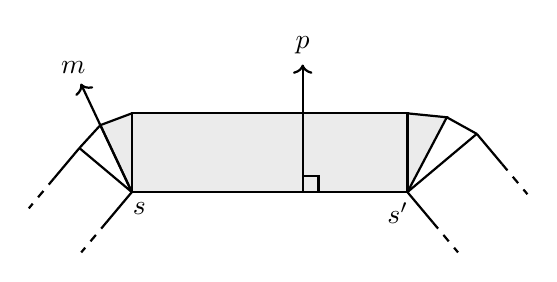
\begin{tikzpicture}

%line info
\def\len{3.5}
\def\theta{50}
\def\w{1}
\def\ratio{1.15}
\def\clenl{0.5}
\def\clenr{0.5}
\def\right{0.2}
%cap points
\coordinate (C)  at (-0.4,\w-0.15);
\coordinate (C') at (\len+0.5,\w-0.05);
%coordinates
\coordinate (B)  at (0,0);
\coordinate (R)  at (0,\w);
\coordinate (B') at (\len,0);
\coordinate (R') at (\len,\w);
\coordinate (N)  at ({-\w/\ratio*sin(\theta)},{\w/\ratio*cos(\theta)});
\coordinate (N') at ({\len+\w*\ratio*sin(\theta)},{\w*\ratio*cos(\theta)});

%fill
\fill[color=black!8!white] (B)  rectangle (R');
\fill[color=black!8!white] (R)  -- (C)  -- (B);
\fill[color=black!8!white] (R') -- (C') -- (B');

%draw edges
\draw[thick] (B)  rectangle (R');
\draw[thick] (B)  -- (N);
\draw[thick] (B') -- (N');
\foreach \x/\y in {0/0,{-\w/\ratio*sin(\theta)}/{\w/\ratio*cos(\theta)}}{
    \draw[thick] ({\x},{\y}) -- ({\x-\clenl*cos(\theta)},{\y-\clenl*sin(\theta)});
    \draw[thick,dashed] ({\x-\clenl*cos(\theta)},{\y-\clenl*sin(\theta)}) -- ({\x-\clenl*2*cos(\theta)},{\y-\clenl*2*sin(\theta)});
}
\foreach \x/\y in {\len/0,{\len+\w*\ratio*sin(\theta)}/{\w*\ratio*cos(\theta)}}{
    \draw[thick] ({\x},{\y}) -- ({\x+\clenr*cos(\theta)},{\y-\clenr*sin(\theta)});
    \draw[thick,dashed] ({\x+\clenr*cos(\theta)},{\y-\clenr*sin(\theta)}) -- ({\x+\clenr*2*cos(\theta)},{\y-\clenr*2*sin(\theta)});
}
\draw[thick] (R)  -- (C)  -- (B)  node[anchor=90+\theta/2]{$s$};
\draw[thick] (R') -- (C') -- (B') node[anchor=90-\theta/2]{$s'$};
\draw[thick] (N)  -- (C);
\draw[thick] (N') -- (C');
%draw arrows
\draw[thick,->] ({0.62*\len},0) -- ({0.62*\len},{1.62*\w}) node[anchor=south]{$p$};
\draw[thick] ({0.62*\len},\right) -- ({0.62*\len+\right},\right) -- ({0.62*\len+\right},0);
\draw[thick,->] (B) -- ($(B)+1.62*(C)$) node[anchor=-90+\theta/2]{$m$};

\end{tikzpicture}
\end{figure}

%%%%%%%%%%%%%%%%%%%%%%%%%%%%%%%%%%%%%%%%%%%%%%%%%%

\begin{figure}[h]
\centering
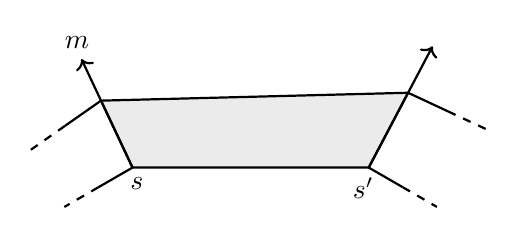
\begin{tikzpicture}

%line info
\def\len{3}
\def\theta{30}
\def\w{1}
\def\ratio{1.15}
\def\clenl{0.5}
\def\clenr{0.5}
\def\right{0.2}
%cap points
\coordinate (C)  at (-0.4,\w-0.15);
\coordinate (C') at (\len+0.5,\w-0.05);
%coordinates
\coordinate (B)  at (0,0);
\coordinate (B') at (\len,0);
\coordinate (N)  at ({-\w/\ratio*sin(\theta)},{\w/\ratio*cos(\theta)});
\coordinate (N') at ({\len+\w*\ratio*sin(\theta)},{\w*\ratio*cos(\theta)});

%fill
\fill[color=black!8!white] (B) -- (C) -- (C') -- (B') -- cycle;

%draw edges
\draw[thick] (B) node[anchor=90+\theta/2]{$s$} -- (C) -- (C') -- (B') node[anchor=90-\theta/2]{$s'$} -- cycle;
\foreach \x/\y [count = \i] in {0/0,{-0.4}/{\w-0.15}}{
    \def\ttheta{\theta+(\i-1)*5}
    \def\tlen{(\clenl+(\i-1)*0.06)}
    \draw[thick] ({\x},{\y}) -- ({\x-\tlen*cos(\ttheta)},{\y-\tlen*sin(\ttheta)});
    \draw[thick,dashed] ({\x-\tlen*cos(\ttheta)},{\y-\tlen*sin(\ttheta)}) -- ({\x-\tlen*2*cos(\ttheta)},{\y-\tlen*2*sin(\ttheta)});
}
\foreach \x/\y [count = \i] in {\len/0,{\len+0.5}/{\w-0.05}}{
    \def\ttheta{\theta-(\i-1)*5}
    \def\tlen{(\clenr+(\i-1)*0.06)}
    \draw[thick] ({\x},{\y}) -- ({\x+\tlen*cos(\ttheta)},{\y-\tlen*sin(\ttheta)});
    \draw[thick,dashed] ({\x+\tlen*cos(\ttheta)},{\y-\tlen*sin(\ttheta)}) -- ({\x+\tlen*2*cos(\ttheta)},{\y-\tlen*2*sin(\ttheta)});
}
%draw arrows
\draw[thick,->] (B)  -- ($(B)+1.62*(C)$) node[anchor=-90+\theta/2]{$m$};
\draw[thick,->] (B') -- ($1.62*(C')-0.62*(B')$);

\end{tikzpicture}
\end{figure}

%%%%%%%%%%%%%%%%%%%%%%%%%%%%%%%%%%%%%%%%%%%%%%%%%%
\fi
\begin{figure}[h]
\centering
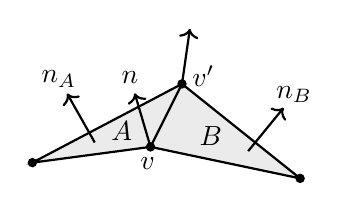
\begin{tikzpicture}

\def\size{0.06}

\coordinate (A) at ( 0.0, 0.0);
\coordinate (B) at ( 0.4, 0.8);
\coordinate (C) at (-1.5,-0.2);
\coordinate (D) at ( 1.9,-0.4);
\coordinate (NV)  at (-0.2, 0.68);
\coordinate (NV') at ( 0.1, 0.7);
\coordinate (NA)  at (-0.35, 0.62);
\coordinate (NB)  at ( 0.45, 0.55);

\fill[color=black!8!white] (A) -- (C) -- (B) -- (D);
\fill[color=black] (A) circle (\size); \fill[color=black] (B) circle (\size); \fill[color=black] (C) circle (\size); \fill[color=black] (D) circle (\size);

\draw[thick] (A) node[anchor=80]{$v$} -- (B) node[anchor=-160]{$v'$} -- (C) -- (A) -- (D) -- (B);
\draw[thick,->] (A) -- ($(A)+(NV)$) node[pos=1.3]{$n$};
\draw[thick,->] (B) -- ($(B)+(NV')$);%node[anchor=-110]{$n_B$};
\draw[thick,->] ($0.38*(B)+0.62*(C)-0.2*(NA)$) -- ($0.38*(B)+0.62*(C)+0.8*(NA)$) node[pos=1.3]{$n_A$};
\draw[thick,->] ($0.38*(B)+0.62*(D)-0.2*(NB)$) -- ($0.38*(B)+0.62*(D)+0.8*(NB)$) node[pos=1.3]{$n_B$};

\node at ($1/3*(A)+1/3*(B)+1/3*(C)$) {$A$};
\node at ($1/3*(A)+1/3*(B)+1/3*(D)$) {$B$};

\end{tikzpicture}
\end{figure}

%%%%%%%%%%%%%%%%%%%%%%%%%%%%%%%%%%%%%%%%%%%%%%%%%%

\begin{figure}[h]
\centering
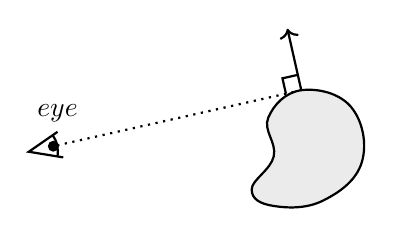
\begin{tikzpicture}

\pgfmathsetmacro{\arrowlen}{0.8}
\pgfmathsetmacro{\right}{0.2}
\pgfmathsetmacro{\eyeX}{-3.1}
\pgfmathsetmacro{\eyeY}{-0.7}

\def\len{sqrt(\eyeX*\eyeX+\eyeY*\eyeY)}
\coordinate (E) at (\eyeX, \eyeY);
\coordinate (OE) at ({\eyeX/\len},{\eyeY/\len});
\coordinate (OP) at ({\eyeY/\len}, {-\eyeX/\len});

\draw[thick,dotted] (E) -- (0,0);
\draw[thick,->] (0,0) -- ($\arrowlen*(OP)$);
\draw[thick] ($\right*(OE)$) -- ($\right*(OE)+\right*(OP)$) -- ($\right*(OP)$);
%\draw[thick] plot[smooth cycle,tension=0.7] coordinates {(0,0) (0.9,-0.3) (1.1,-1.3) (0.4,-2) (-0.5,-2.1) (-0.9,-1.8) (-0.5,-1.2) (-0.6,-0.5)};
\fill[color=black!8!white] plot[smooth cycle,tension=0.7] coordinates {(0,0) (0.63,-0.21) (0.77,-0.91) (0.28,-1.4) (-0.35,-1.47) (-0.63,-1.26) (-0.35,-0.84) (-0.42,-0.35)};
\draw[thick] plot[smooth cycle,tension=0.7] coordinates {(0,0) (0.63,-0.21) (0.77,-0.91) (0.28,-1.4) (-0.35,-1.47) (-0.63,-1.26) (-0.35,-0.84) (-0.42,-0.35)};

\pgfmathsetmacro{\eye}{0.37}
\pgfmathsetmacro{\width}{22}
\def\angle{atan(\eyeY/\eyeX)}

\coordinate (B) at ($(E)+\eye*(OE)$);
\coordinate (L) at ({cos(\angle-\width)},{sin(\angle-\width)});
\coordinate (U) at ({cos(\angle+\width)},{sin(\angle+\width)});

\draw[thick] ($(B)+1.2*\eye*(L)$) -- (B) -- ($(B)+1.2*\eye*(U)$) node[anchor=-90]{$eye$};
\draw[thick] (E) arc (\angle:\angle+\width:\eye);
\draw[thick] (E) arc (\angle:\angle-\width:\eye);
\fill[color=black] ($(E)+0.05*(OE)$) circle (0.07);

\end{tikzpicture}
\end{figure}

%%%%%%%%%%%%%%%%%%%%%%%%%%%%%%%%%%%%%%%%%%%%%%%%%%

\end{document}
